\chapter{Mass fit to \decay{\Bp}{\Dsp\Kp\Km} candidates} 
\label{ch:B2DsKK}

\minitoc

In this chapter the methodology used to search for \decay{\Bp}{\Dsp\Kp\Km} decays is described.
The branching fraction $\BF(\decay{\Bp}{\Dsp\Kp\Km})$ is determined by measuring the ratio of \decay{\Bp}{\Dsp\Kp\Km} and \decay{\Bp}{\Dsp\Dzb} yields. 
This is corrected by the ratio of efficiencies for the two modes and multiplied by the externally measured branching fractions for \decay{\Bp}{\Dsp\Dzb} and \decay{\Dzb}{\Kp\Km} decays.

\begin{multline}
\BF(\decay{\Bp}{\Dsp\Kp\Km}) = \frac{N(\decay{\Bp}{\Dsp\Kp\Km})}{N(\decay{\Bp}{\Dsp\Dzb})} \times  \frac{\epsilon(\decay{\Bp}{\Dsp\Dzb})}{\epsilon(\decay{\Bp}{\Dsp\Kp\Km})}\\ 
\times \BF(\decay{\Bp}{\Dsp\Dzb}) \times \BF(\decay{\Dzb}{\Kp\Km}) 
\end{multline}

The fit models used to extract the yields $N(\decay{\Bp}{\Dsp\Kp\Km})$ and $N(\decay{\Bp}{\Dsp\Dzb})$ are described in Section~\ref{sec:B2DsKK_fitcomps}, the efficiency corrections are described in Section~\ref{sec:B2DsKK_effcorrection} and the resulting calculation of the branching fraction is in Section~\ref{sec:B2DsKK_results}.


\section{Fit components}
\label{sec:B2DsKK_fitcomps}

In order to extract the yields of \decay{\Bp}{\Dsp\Dzb} and \decay{\Bp}{\Dsp\Kp\Km} decays the invariant mass distributions for the processes contributing within the invariant mass range are parametrised with probability density functions (PDFs).
Both the signal and normalisation channels are fitted within the same \Bp meson invariant mass range 5100--5900\mevcc. This is sufficiently wide to allow the contributions from different background modes to be distinguished and accurately extrapolated into the signal region.  

{\color{Red}
\begin{itemize}
\item any other quantities that might be needed
\end{itemize}
}


\subsection{Signal and normalisation decays}
\label{sec:B2DsKK_sigcomps}

The invariant mass distribution of \decay{\Bp}{\Dsp\Dzb} and \decay{\Bp}{\Dsp\Kp\Km} decays are parametrised as the sum of two Crystal Ball (CB) functions.
The CB function consists of a Gaussian function with a power-law tail and is typically used to parametrise losses due to radiative processes.
This is defined as
\begin{equation}
\text{CB}(m,\mu,\sigma,n,\alpha) = \left \{
  \begin{aligned}
    &e^{-\frac{1}{2} \left(\frac{m-\mu}{\sigma}\right)^2}, && \text{if}\ \left(\frac{m-\mu}{\sigma}\right) < -|\alpha|\\
    &\frac{\left(\frac{n}{|\alpha|}\right)^n\times e ^{-\frac{1}{2}|\alpha|^2} }{\left(\frac{n}{|\alpha|}-|\alpha| - \frac{m-\mu}{\sigma}\right)^n}, && \text{otherwise}
  \end{aligned} \right.
\end{equation} 

where $\mu$, $\sigma$, $n$ and $\alpha$ are adjustable parameters and $m$ is the \B meson invariant mass observable.
The sum of two CB functions is constructed with a variable fraction $f_\sigma$ assigned to the CB function with the narrower width,
\begin{equation}
\text{DCB}(m,\mu,\sigma_1,\sigma_2,n,\alpha) = f_\sigma \times \text{CB}(m,\mu,\sigma_1,n,\alpha) + (1-f_\sigma) \times \text{CB}(m,\mu,\sigma_2,n,\alpha),
\label{eq:DoubleBD}
\end{equation}
where the same tail parameters, $n$ and $\alpha$ are used for both functions, but the widths, $\sigma_1$ and $\sigma_2$, are allowed to be different (with $\sigma_1 < \sigma_2$).
As both CB shapes have the same parameter $\alpha$, the tails are constrained to be on the same side.
Values for the adjustable parameters are determined from fits to simulated decays passing the selection requirements applied to the data. 
%These are determined separately for the different \Dsp decay modes. 
However, a number of parameters are not completely constrained from the simulations. The mean position $\mu$ is allowed vary freely in the fit to data, as is the narrowest CB width of the normalisation and signal decays. 
%The ratios $\sigma_1/\sigma_2$ and $\sigma_{1}(\Dsp\phi) / \sigma_{1}(\Dsp\Dzb)$ are fixed from simulations.
The tail parameters $n$ and $\alpha$ are highly correlated, therefore the value of $n$ is fixed to unity in both the fits to simulations and data. The values determined from simulations for \decay{\Bp}{\Dsp\Dzb} and \decay{\Bp}{\Dsp\Kp\Km} decays are tabulated in Table~\ref{tab:B2DsKK_signal_mc_fits} and the results of the corresponding fits are shown in Fig.~\ref{fig:B2DsKK_signal_fits}.


%%%%%%%%%%%%%%%%%%%%%%%%%%%%%%%%%%%%%%%%%%%%%%%%%%%%%%%%%% 
\begin{table}[h]
\centering
\begin{tabular}{ c c }
\hline
Parameter                   & Value \\
\hline
\multicolumn{2}{c} {\decay{\Bp}{\Dsp\Kp\Km}}\\

\hline
$\sigma_1/\sigma_2$         & 0.53 $\pm$ 0.02  \\
$f_\sigma$                  & 0.87 $\pm$ 0.02  \\
$\alpha$                    & 2.60 $\pm$ 0.03  \\
$n$                         & 1 $\pm$ 0        \\
\hline
\multicolumn{2}{c} {\decay{\Bp}{\Dsp\Dzb}}\\
\hline
$\sigma_1/\sigma_2$         & 0.60 $\pm$ 0.03    \\
$f_\sigma$                  & 0.66 $\pm$ 0.12    \\
$\alpha$                    & 2.67 $\pm$ 0.12    \\
$n$                         & 1 $\pm$ 0          \\
\hline
\end{tabular}
\caption{Fixed values obtained in fits to simulations used in the model for the signal and normalisation PDFs.} 
\label{tab:B2DsKK_signal_mc_fits}  
\end{table}
%%%%%%%%%%%%%%%%%%%%%%%%%%%%%%%%%%%%%%%%%%%%%%%%%%%%%%%%%% 

%%%%%%%%%%%%%%%%%%%%%%%%%%%%%%%%%%%%%%%%%%%%%%%%%%%%%%%%%%
\begin{figure}[!h]
    \centering
    \begin{subfigure}[t]{1.0\textwidth}
        \includegraphics[width=0.48\textwidth]{figs/B2DsKK/Plot_Signal_Fit_All_B2DsKK_Ds2KKPi.pdf}
        \includegraphics[width=0.48\textwidth]{figs/B2DsKK/Plot_Signal_Fit_All_B2DsD0_Ds2KKPi.pdf}
    \end{subfigure}\\
    \caption{Invariant mass fits to signal (left) and normalisation (right) channel simulation samples.}
    \label{fig:B2DsKK_signal_fits}   
\end{figure}
%%%%%%%%%%%%%%%%%%%%%%%%%%%%%%%%%%%%%%%%%%%%%%%%%%%%%%%%%%


\subsection{Partially reconstructed backgrounds}
\label{sec:B2DsKK_partrecocomps}

Partially reconstructed decays are those in which the five final state particles combined in the signal mode are only a subset of a background mode's final state.
Decays of \B mesons can contribute at lower invariant masses below the signal peak when one or more the decay products have not been reconstructed. 
For decays to contribute within the fitted \Bp invariant mass window, the particle or particles that have not been reconstructed must be fairly low-momentum (soft) such that the invariant mass of the remaining particles is large.

\subsubsection{Backgrounds to the normalisation channel}

The low invariant mass region of the \Dsp\Dzb spectrum is populated by decays of \Bp mesons to combinations of \D and excited \D mesons. These \Dstarzb and \Dss mesons decay strongly to a ground state \Dzb or \Dsp meson and a soft pion or photon. The branching fractions for these decays are listed in Table~\ref{tab:dstar_BFs}.


%%%%%%%%%%%%%%%%%%%%%%%%%%%%%%%%%%%%%%%%%%%%%%%%%%%%%%%%%% 
\begin{table}[h]
\centering
\begin{tabular}{ l c }

\hline
Decay                           & Branching fraction \\ 
\hline
\decay{\Dstarzb}{\Dzb\Pgamma}   &   $(64.7\pm0.9)\%$ \\
\decay{\Dstarzb}{\Dzb\piz}      &   $(35.3\pm0.9)\%$ \\
\decay{\Dssp}{\Dsp\Pgamma}        &   $(93.5\pm0.7)\%$ \\
\decay{\Dssp}{\Dsp\piz}           &   $(5.8\pm0.7)\%$ \\
\hline

\end{tabular}
\caption{Branching fractions for excited charm mesons \cite{PDG2016}. } 
\label{tab:dstar_BFs}  
\end{table}
%%%%%%%%%%%%%%%%%%%%%%%%%%%%%%%%%%%%%%%%%%%%%%%%%%%%%%%%%% 

The excited charm mesons \Dstarzb and \Dss {\color{Red}(be more specific)} are vector ($J^{P} = 1^{-}$) mesons. The partially reconstructed invariant mass of the \Dsp and \Dzb mesons can vary depending on the spin of the missed particle.
Analytical PDFs are used to account for the spin of the missed particle. These were developed by considering the helicity angle 




{\color{Red}
\begin{itemize}
\item add formulas for hills and horns
\end{itemize}
}



%%%%%%%%%%%%%%%%%%%%%%%%%%%%%%%%%%%%%%%%%%%%%%%%%%%%%%%%%%
\begin{figure}[!h]
    \centering
    \includegraphics[width=0.80\textwidth]{figs/B2DsPhi/DsD0_part_reco_Shapes.pdf}
    \caption{Partially reconstructed \Dsp\Dzb shapes.}
    \label{fig:B2DsPhi_DsD0_partreco}   
\end{figure}
%%%%%%%%%%%%%%%%%%%%%%%%%%%%%%%%%%%%%%%%%%%%%%%%%%%%%%%%%%





\subsubsection{Backgrounds to the signal channel}

The signal channel receives contributions at low invariant mass from a number of different decays. 
All modes considered involve a \Bs or \Bz meson decay in which one or more soft decay products have not been reconstructed.

\begin{description}
\item \decay{\Bsb}{\Dsp\Km\Kstarz}: this decay can form a background to the \decay{\Bp}{\Dsp\Kp\Km} signal when a soft pion from the \decay{\Kstarz}{\Kp\pim} decay is not reconstructed. The PDF for this background is determined from a sample of fully reconstructed simulated events that have been processed using the same procedure as the signal decays. The PDF is created using a kernel estimation technique~\cite{Cranmer:2000du} implemented in the \texttt{RooKeysPDF} class within \texttt{RooFit}. The resulting PDF is shown in Fig.~\ref{fig:B2DsKK_part_reco_backgrounds}.
\item \decay{\Bsb}{\Dssp\Km\Kstarz}: Similarly this decay can form a background at low invariant mass when a soft neutral particle is not reconstructed in the \decay{\Dssp}{\Dsp X} decay in addition to the pion from the \Kstarz. This PDF is also determined using the \texttt{RooKeysPDF} class and shown in Fig.~\ref{fig:B2DsKK_part_reco_backgrounds}.
\item \decay{\Bsb}{\Dsp\Dsm}: decays of this 
\item \decay{\Bzb}{\Dsp\Dm}: decays of this
\item \decay{\Bsb}{\Dssp\Dsm}: decays of this 

\end{description}


%%%%%%%%%%%%%%%%%%%%%%%%%%%%%%%%%%%%%%%%%%%%%%%%%%%%%%%%%%
\begin{figure}[!h]
    \centering
    \begin{subfigure}[t]{0.49\textwidth}
        \includegraphics[width=1.0\textwidth]{figs/B2DsKK/Bs2Dsa1_4800_5900_Shape.pdf}
        \caption{\decay{\Bsb}{\Dsp\Km\Kstarz} }
    \end{subfigure}
    \begin{subfigure}[t]{0.49\textwidth}
        \includegraphics[width=1.0\textwidth]{figs/B2DsKK/Bs2DsstKKst_4800_5900_Shape.pdf}
        \caption{\decay{\Bsb}{\Dssp\Km\Kstarz}}
    \end{subfigure}
    \begin{subfigure}[t]{0.49\textwidth}
        \includegraphics[width=1.0\textwidth]{figs/B2DsKK/Bs2DsDs_4800_5900_Shape.pdf}
        \caption{\decay{\Bsb}{\Dsp\Dsm} }
    \end{subfigure}
    \begin{subfigure}[t]{0.49\textwidth}
        \includegraphics[width=1.0\textwidth]{figs/B2DsKK/Bs2DsstDs_4800_5900_Shape.pdf}
        \caption{\decay{\Bsb}{\Dssp\Dsm} }
    \end{subfigure}
    \caption{Partially reconstructed mass shapes}
    \label{fig:B2DsKK_part_reco_backgrounds}   
\end{figure}
%%%%%%%%%%%%%%%%%%%%%%%%%%%%%%%%%%%%%%%%%%%%%%%%%%%%%%%%%%

{\color{Red}
\begin{itemize}
\item plots of part reco shapes
\end{itemize}
}

\subsection{Combinatorial  background}
\label{sec:B2DsKK_combcomps}

The dominant source of background under the signal peak is due to combinations of unrelated tracks. This combinatorial background is modelled using an exponential function with a single degree of freedom controlling the effective slope of the function. 

{\color{Red}
\begin{itemize}
\item check what happens to the slopes
\end{itemize}
}
%This slope is shared between the normalisation and signal channels, and between different \Dsp decay modes. This adds stability to the fit.


\section{Fit strategy}
\label{sec:B2DsKK_fitstrategy}
The search for $\decay{\Bp}{\Dsp\Kp\Km}$ involves two independent maximum likelihood fits for the signal and normalisation channels. The $\decay{\Bp}{\Dsp\Kp\Km}$ yield is corrected on a per-candidate basis to account for the phase-space dependence of the signal efficiencies in this three-body decay. 


{\color{Red}
\begin{itemize}
\item How yield is corrected, introduce sWeights
\item $m(\Kp\Km)$ range that goes into fit
\end{itemize}
}



\section{Fit validation}
\label{sec:B2DsKK_fitvalidation}

{\color{Red}
\begin{itemize}
\item Toys for signal and normalisation
\item why it doesn't matter that norm yield have wrong pulls
\item 
\end{itemize}
}

\section{Normalisation and signal fits}

The results of the two fits to signal and normalisation candidates are shown in Figs.~\ref{fig:fit_B2DsD0} and \ref{fig:fit_B2DsKK}. The total fit model is overlaid upon the data distributions. Additionally the contributions from each different component in the model is included as detailed in the legends.

%%%%%%%%%%%%%%%%%%%%%%%%%%%%%%%%%%%%%%%%%%%%%%%%%%%%%%%%%%
\begin{figure}[!h]
    \centering
    \includegraphics[width=0.8\textwidth]{figs/B2DsKK/Fit_DsD0.pdf}
    \caption{Invariant mass fit to \decay{\Bp}{\Dsp\Dzb} candidates.}
    \label{fig:fit_B2DsD0}   
\end{figure}
%%%%%%%%%%%%%%%%%%%%%%%%%%%%%%%%%%%%%%%%%%%%%%%%%%%%%%%%%%

%%%%%%%%%%%%%%%%%%%%%%%%%%%%%%%%%%%%%%%%%%%%%%%%%%%%%%%%%%
\begin{figure}[!h]
    \centering
    \includegraphics[width=0.8\textwidth]{figs/B2DsKK/Fit_DsKK.pdf}
    \caption{Invariant mass fit to \decay{\Bp}{\Dsp\Kp\Km} candidates.}
    \label{fig:fit_B2DsKK}   
\end{figure}
%%%%%%%%%%%%%%%%%%%%%%%%%%%%%%%%%%%%%%%%%%%%%%%%%%%%%%%%%%


\section{Efficiency corrections}
\label{sec:B2DsKK_effcorrection}

{\color{Red}
\begin{itemize}
\item plots of eff across dalitz plot
\item studies of BDT eff ratio 
\end{itemize}
}


\section{Systematic uncertainties}
\label{sec:B2DsKK_systuncertainy}


\section{Results}
\label{sec:B2DsKK_results}



{\color{Red}
\begin{itemize}
\item Copy most of results section from paper
\item equations
\item include sWeighted, eff corrected plots
\item include dalitz plot
\end{itemize}
}

{\color{Blue}
The fit to $\decay{\Bp}{\Dsp\Kp\Km}$ candidates finds a total yield of $N(\decay{\Bp}{\Dsp\Kp\Km}) = 443 \pm 29 $ candidates. 
This constitutes the first observation of this decay mode.
The branching fraction is calculated as
\begin{equation}
\mathcal{B}(\decay{\Bp}{\Dsp\Kp\Km}) = \frac{ N_{\text{corr}}(\decay{\Bp}{\Dsp\Kp\Km}) }{ N(\decay{\Bp}{\Dsp\Dzb}) } \times \mathcal{B}(\decay{\Bp}{\Dsp\Dzb}) \times \mathcal{B}(\decay{\Dzb}{\Kp\Km})
\label{eq:DsKKBranchingfraction}
\end{equation}
\noindent where $N(\decay{\Bp}{\Dsp\Dzb})$ is the yield of normalisation decays, and $N_{\text{corr}}(\decay{\Bp}{\Dsp\Kp\Km})$ is defined to be
\begin{equation}
N_{\text{corr}}(\decay{\Bp}{\Dsp\Kp\Km}) =  \sum\limits_{i} \frac{W_{i}}{\epsilon^{\text{ratio}}_{i}},
\end{equation}
\noindent where $W_{i}$ is the per-candidate weight, as determined by the \sPlot technique for candidate $i$; and $\epsilon^{\text{ratio}}_{i}$ represents the relative efficiency of the signal and normalisation modes $\epsilon_{i}(\decay{\Bp}{\Dsp\Kp\Km})/\epsilon(\decay{\Bp}{\Dsp\Dzb})$ in the relevant bin of the $\decay{\Bp}{\Dsp\Kp\Km}$ Dalitz plot. The corrected yield ratio can be expressed as the ratio of signal and normalisation branching fractions using Eq.~\ref{eq:DsKKBranchingfraction}. The value is measured to be 
\begin{equation*}
\frac{ N_{\text{corr}}(\decay{\Bp}{\Dsp\Kp\Km}) }{ N(\decay{\Bp}{\Dsp\Dzb}) } = \frac{\mathcal{B}(\decay{\Bp}{\Dsp\Kp\Km})}{\mathcal{B}(\decay{\Bp}{\Dsp\Dzb})\mathcal{B}(\decay{\Dzb}{\Kp\Km})}  = 0.197 \pm 0.015 \pm 0.017, 
\end{equation*}
where the first uncertainty is statistical, and the second is systematic.
The branching fraction for $\decay{\Bp}{\Dsp\Kp\Km}$ decays is determined to be 

\begin{equation*}
\mathcal{B}(\decay{\Bp}{\Dsp\Kp\Km}) = (7.1 \pm 0.5 \pm 0.6 \pm 0.7) \times 10^{-6},
\end{equation*}
where the first uncertainty is statistical, the second is systematic and the third from the branching fractions of $\decay{\Dzb}{\Kp\Km}$ and of the normalisation mode $\decay{\Bp}{\Dsp\Dzb}$. 
The values used for the branching fractions are $\mathcal{B}(\decay{\Dz}{\Kp\Km}) = (4.01 \pm 0.07)\times10^{-3}$ and $\mathcal{B}(\decay{\Bp}{\Dsp\Dzb}) = (9.0 \pm 0.9)\times10^{-3}$~\cite{PDG2016}. 
The two-body projections $m(D_{s}^{+}K^{-})$ and $m(K^{+}K^{-})$ are obtained for the signal component using the \sPlot technique, shown in Fig.~\ref{fig:B2DsKK_twobodyprojections}. No significant peak is observed in the \phiz region of the $m(\Kp\Km)$ plot; rather a broad distribution of candidates is found in the region up to $m(\Kp\Km) \simeq 1900 \mevcc$. 
}

%%%%%%%%%%%%%%%%%%%%%%%%%%%%%%%%%%%%%%%%%%%%%%%%%%%%%%%%%%
\begin{figure}[!h]
    \centering
    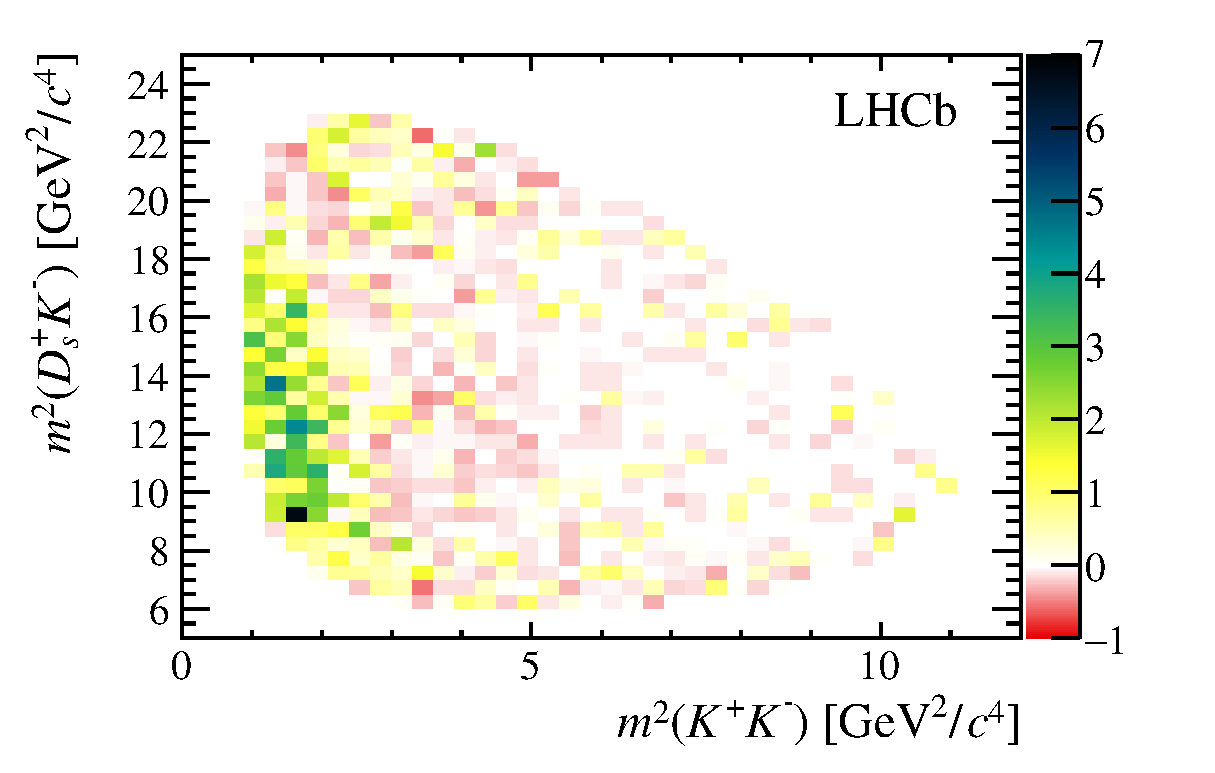
\includegraphics[width=0.8\textwidth]{figs/B2DsKK/Dalitz_plot_sweighted.eps}
    \caption{Dalitz plot}
    \label{fig:B2DsKK_Dalitzplot}   
\end{figure}
%%%%%%%%%%%%%%%%%%%%%%%%%%%%%%%%%%%%%%%%%%%%%%%%%%%%%%%%%%

%%%%%%%%%%%%%%%%%%%%%%%%%%%%%%%%%%%%%%%%%%%%%%%%%%%%%%%%%%
\begin{figure}[!h]
    \centering
    \begin{subfigure}[t]{0.49\textwidth}
        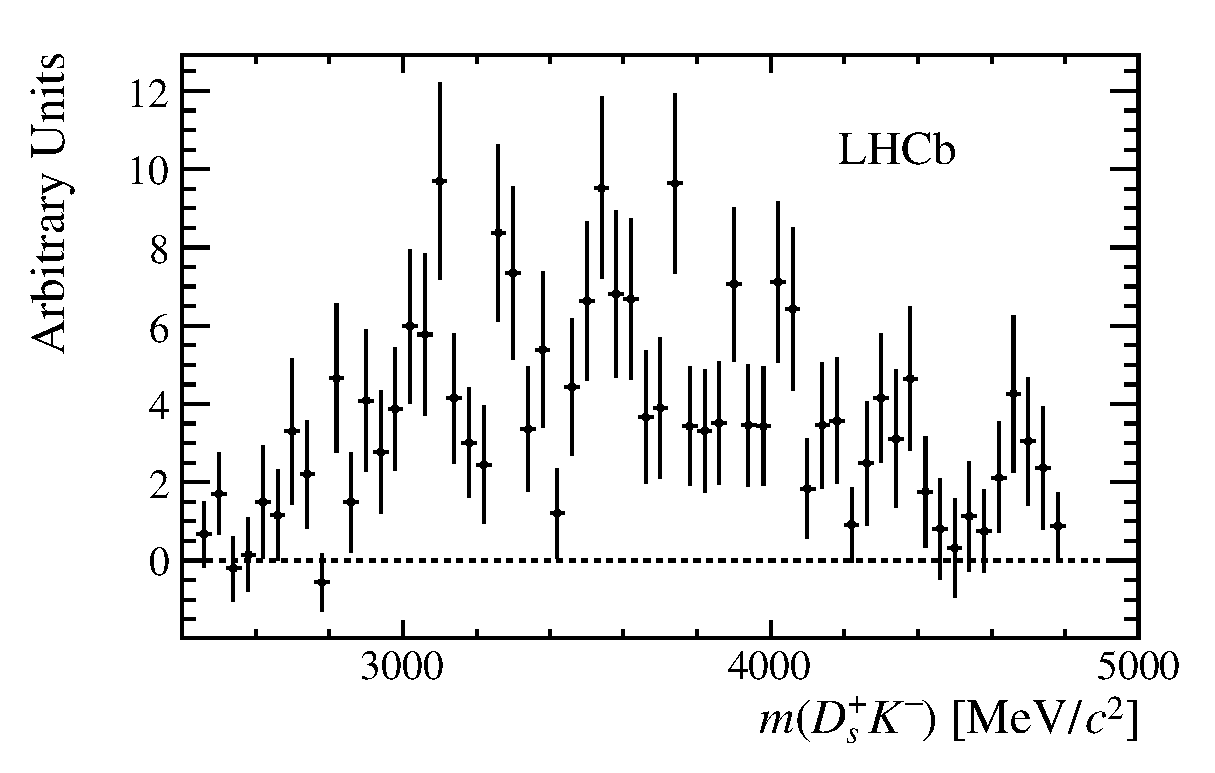
\includegraphics[width=1.0\textwidth]{figs/B2DsKK/DsKm_mass_sweighted.eps}
        %\caption{Normalisation without selection}
    \end{subfigure}
    \begin{subfigure}[t]{0.49\textwidth}
        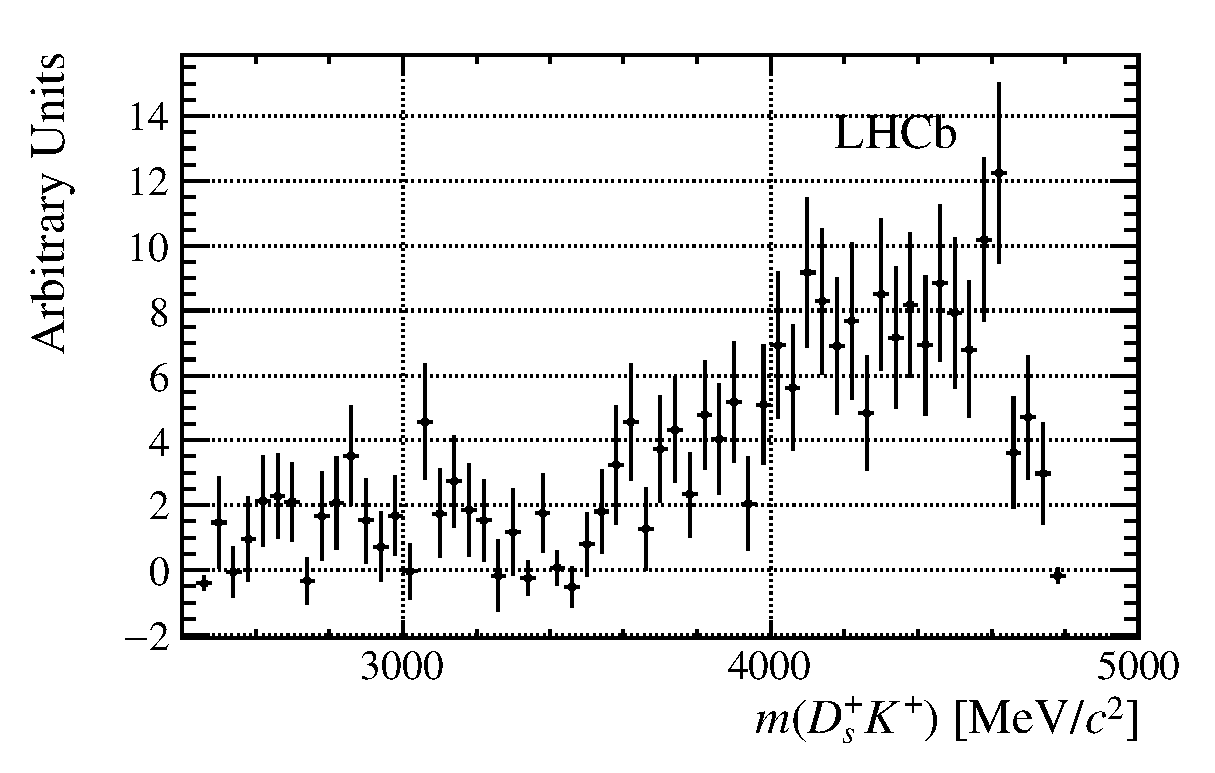
\includegraphics[width=1.0\textwidth]{figs/B2DsKK/DsKp_mass_sweighted.eps}
        %\caption{Normalisation without selection}
    \end{subfigure}
    \begin{subfigure}[t]{0.49\textwidth}
        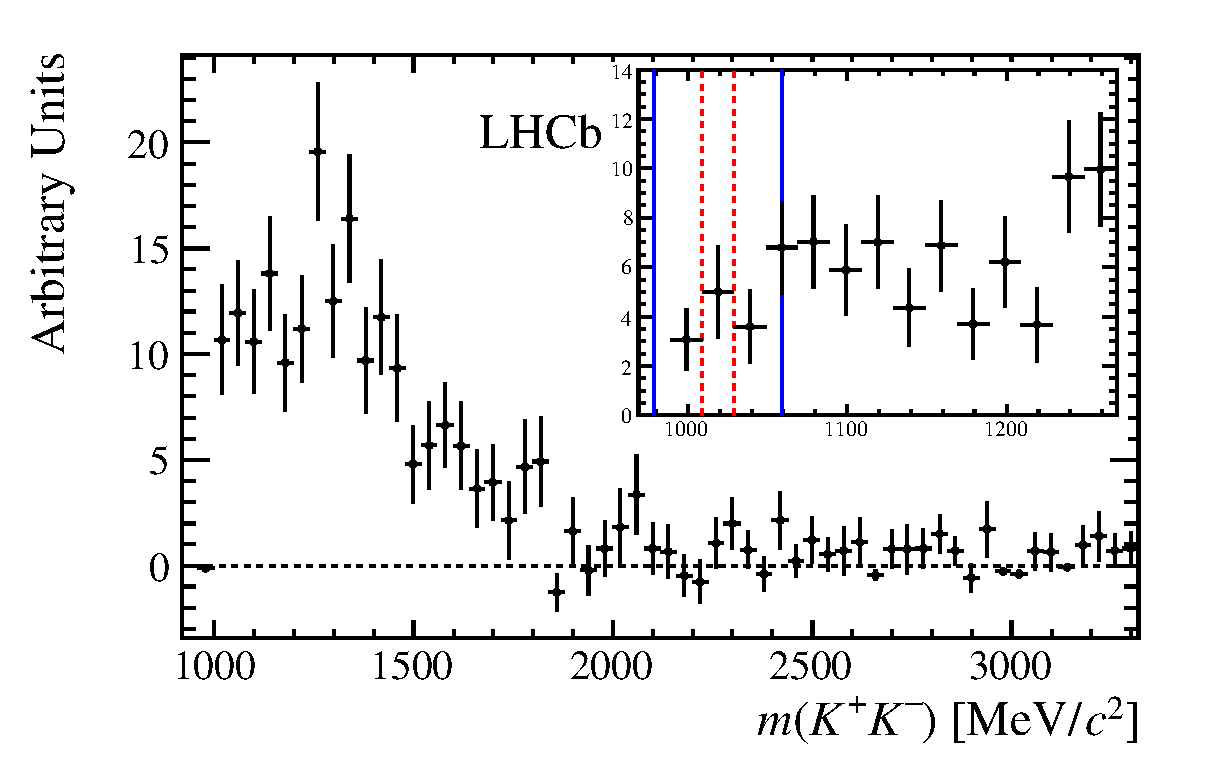
\includegraphics[width=1.0\textwidth]{figs/B2DsKK/phi_mass_sweighted.eps}
        %\caption{Normalisation without selection}
    \end{subfigure}
    \caption{Two-body mass projections}
    \label{fig:B2DsKK_twobodyprojections}
\end{figure}
%%%%%%%%%%%%%%%%%%%%%%%%%%%%%%%%%%%%%%%%%%%%%%%%%%%%%%%%%%

